\documentclass[a4paper,man,natbib,floatsintext,12pt]{apa7}

\usepackage[english]{babel} %character and hyphenation rules specific to the language you choose
%\usepackage[utf8x]{inputenc}
\usepackage{graphicx}
\usepackage{color}
\usepackage{tikz}
\usepackage{amsmath}
\usepackage{blindtext}
\usepackage{tabularx} %great for APA-style Tables
\usepackage{siunitx} % Required for good table alignmen
\sisetup{
  round-mode          = places, % Rounds numbers
  round-precision     = 2, % to 2 places
}
\usepackage{multirow}
\usepackage{booktabs}
\usepackage{wrapfig}
\usepackage[utf8]{inputenc}
\usepackage{textgreek} % for Greek letters in text
\usetikzlibrary{shapes,decorations,arrows,calc,arrows.meta,fit,positioning}
\tikzset{
    -Latex,auto,node distance =1 cm and 1 cm,semithick,
    latent/.style ={ellipse, draw, minimum width = 0.7 cm},
    observed/.style ={rectangle, draw},
    bidirected/.style={Latex-Latex,dashed},
    el/.style = {inner sep=2pt, align=left, sloped}
}
\newcommand{\sigFtest}[4]{\textit{F}(#1,#2) = #3, \textit{p}$<$#4}
\newcommand{\nonsigFtest}[3]{\textit{F}(#1,#2) = #3, \textit{p}$>$.05}


\title{Psychometric Validation of the Mandarin Version of the Duke Misophonia Questionnaire}
\shorttitle{Validation of the Mandarin DMQ}
\author{Abby Wang}
\affiliation{College of William \& Mary}
\journal{Journal of Affective Disorder}
\abstract{Misophonia is a condition characterized by strong emotional and physiological responses to specific trigger sounds. While extensively studied in Western populations, research on misophonia in Chinese populations remains limited, possibly due to the lack of assessment instruments. This study aimed to develop and validate a Mandarin version of the Duke Misophonia Questionnaire (DMQ) for use in China. A sample of 704 Mandarin-speaking participants completed the DMQ alongside other psychometric instruments assessing related constructs, including anxiety, depression, hyperacusis, and obsessive-compulsive symptoms. Item Response Theory (IRT) analysis confirmed a predominantly comparable structure between the Mandarin and English versions, though some subscales exhibited cross-cultural differences. Reliability analyses indicated strong internal consistency, and validity assessments demonstrated robust convergent and discriminant validity. Notably, affective and cognitive responses to misophonic triggers showed significant correlations with anxiety and depressive symptoms, highlighting potential shared mechanisms. These findings support the Mandarin DMQ as a reliable and valid tool for assessing misophonia in Chinese populations and provide insights into cultural influences on misophonia symptomatology. Future research should further explore the role of cultural norms in shaping symptom expression and coping strategies.}
\keywords{Misophonia; Psychometrics; China; Mandarin; Duke Misophonia Questionnaire}
\authornote{This research was funded by the Duke Kunshan University Signature Work Office and Academic Services. The authors extend their sincere gratitude to Dr. Zachary Rosenthal’s research team at the Duke Center for Misophonia and Emotion Regulation for their expert guidance in refining survey translations and selecting appropriate constructs. We are also deeply grateful to Chyi Ricketts and Jason Qiu for their meticulous back-translation work, which added to the linguistic and cultural accuracy of our survey materials. Additionally, we would like to acknowledge Zachary Williams from Vanderbilt University for his insightful feedback on data interpretation. The authors confirm that no generative artificial intelligence tools were used in the drafting of this manuscript, including its text, figures, or any other content.}
\leftheader{Alternate page header in man mode}

%-------------- END PREAMBLE  -------------------


\begin{document}

\maketitle  %Insert my APA style title page

\section{Introduction}

Misophonia is a condition marked by intense negative reactions—emotional, physiological, and behavioral—to specific everyday sounds, such as chewing, breathing, or environmental noises \citep{Jastreboff2001} . These auditory triggers most commonly include eating-related sounds, nasal and throat sounds, and other repetitive noises, with eating sounds frequently reported as the most distressing (\citep{Vitoratou2021a}). Individuals with misophonia often experience acute emotional responses such as anger and disgust, accompanied by physiological symptoms like increased heart rate, sweating, and muscle tension. These reactions can lead to considerable functional impairment, including avoidance behaviors, social withdrawal, and even aggressive outbursts.
Network analysis enables an understanding of the interconnections among subscales, providing insights into which parts of the measure are most central to the others. This study employed network analysis to examine the interconnections among DMQ subscales and identify the most central components of misophonia symptomatology.


\section{Method}
Network analysis was conducted on DMQ data from 144 adults with varying levels of misophonia symptoms. Four network models were examined: overall misophonia, symptoms, beliefs, and impairment. Sex differences were also explored.
\subsection{Participants}
Participants aged 18 years or older and fluent in Mandarin were eligible for inclusion. Exclusion criteria included self-reported severe learning or intellectual disabilities. An information sheet was provided at the start of the survey, and participants gave informed consent before completing the online questionnaires. This work is reviewed and approved by the Duke Kunshan University Institutional Review Board (Ref: 2024SW125). 
\subsection{Materials and Measures}
\textit{Duke Misophonia Questionnaire (DMQ)}
The Duke Misophonia Questionnaire (DMQ) is the first psychometrically validated self-report measure of misophonia developed for an English-speaking population (Rosenthal et al., 2021). The DMQ underwent a rigorous two-phase development process. In Phase 1, items were generated and iteratively refined using input from multiple stakeholders, including misophonia sufferers, their family members, and professional experts. In Phase 2, a large community sample of adults (n = 424) recruited through Amazon’s Mechanical Turk completed DMQ candidate items and other measures for psychometric analyses. 

\textit{Selective Sound Sensitivity Syndrome Scale (S-Five)} 
The Selective Sound Sensitivity Syndrome Scale (S-Five) consists of two sections: S-Five Experiences and S-Five Trigger Checklist. The S-Five Experiences is a 25-item measure designed to assess the severity of misophonia (Vitoratou et al., 2021b). Each item is rated on an 11-point rating scale, ranging from 0 (not at all true) to 10 (completely true), resulting in a total score ranging from 0 to 250. Vitoratou et al. (2023) established a cut-off of 87 or higher on the total score to indicate significant misophonia. In this study, we used a validated Mandarin version for Chinese populations, which, in its original validation (Vitoratou et al., 2022), showed a replicated five-factor structure and demonstrated satisfactory internal consistency across all factors, with both Cronbach’s α and McDonald’s ω coefficients of 0.88 or higher. The S-Five Trigger Checklist (S-Five-T) was developed to assess the nature and intensity of various trigger sounds (Vitoratou et al., 2021b). Designed for flexibility, the S-Five-T allows researchers to adjust the number of triggers used. In this study, we administered the 37 trigger sounds from the original S-Five validation study, which have been validated in a Chinese population, demonstrating acceptable reliability, convergent validity, and discriminant validity (Vitoratou et al., 2022). The original response options for emotional reactions were also retained: no feeling, irritation, distress, disgust, anger, panic, other feelings (negative), and other feelings (positive). For each trigger item, respondents first select their primary emotional reaction and then rate the intensity of that reaction (henceforth, trigger intensity) on a scale from 0 (does not bother me at all) to 10 (unbearable/causes suffering). 


\section{Results}

\subsection{Participant Exclusion and Sample Characteristics}
For our analyses, we excluded participants who responded with "I am not bothered by any sounds or sights associated with sounds," as they were directed to the end of the survey. This decision aligns with DeVellis (2016), as the scale is designed to measure the severity and characteristics of misophonia symptoms. Including respondents who explicitly deny experiencing the core phenomenon would be inconsistent with the scale's intended purpose and would artificially inflate the proportion of zero or near-zero scores, potentially distorting key psychometric properties such as item discrimination and internal consistency. Moreover, validating clinical assessment tools requires evaluating item performance and scale structure using a sample representative of the intended clinical population—in this case, individuals who experience at least minimal sound sensitivity (Streiner et al., 2015). Including participants who report no symptoms would not provide meaningful information about how the scale functions for those it is designed to assess.

\begin{wrapfigure}{r}{0.45\textwidth}     
    \centering       
    \includegraphics[width=0.2\textwidth]{Picture1.png}
    \caption{Geographic distribution of participants across China}
    \label{fig:latbrain}
\end{wrapfigure}

The final sample comprised 704 participants (337 males, 367 females) with a mean age of 25.3 years (SD = 5.94). The majority of participants (n = 615; 87.4\%) had completed an undergraduate degree, reflecting a highly educated sample. In terms of ethnic composition, the sample was predominantly Han Chinese (n = 689; 97.9\%), while the remaining participants belonged to various ethnic minority groups, including Uygur, Yi, Manchu, Tujia, Zhuang, Bai, and Mongolian. Participants were recruited from diverse geographical regions across China, with over 60\% originating from East China and South Central China, ensuring a broad representation of cultural and regional backgrounds (see Figure~\ref{fig:latbrain}).

\subsection{Validation Framework}
The validation framework employed a comprehensive approach examining multiple psychometric properties through a systematic analysis of validity and reliability measures (see Figure~\ref{fig:TikZmodel}).

\begin{figure}[ht!]
\centering
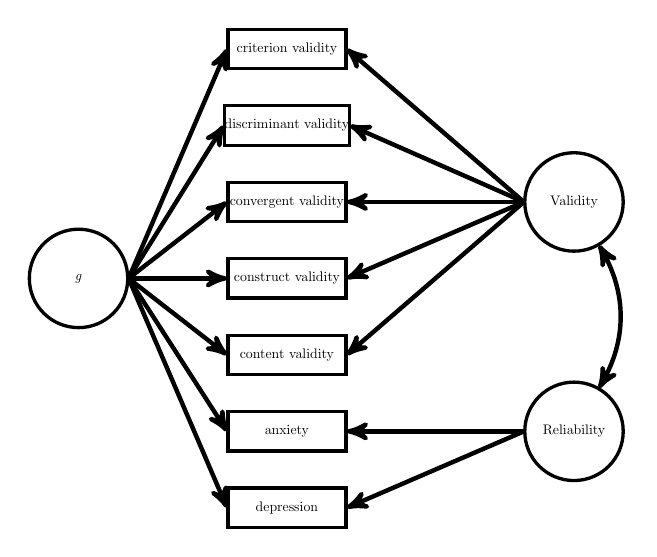
\begin{tikzpicture}[scale=.5,transform shape,auto,node distance=.9cm,
latent/.style={circle,draw,very thick,inner sep=0pt,minimum size=25mm,align=center},
manifest/.style={rectangle,draw,very thick,inner sep=0pt,minimum width=30mm,minimum height=10mm},
paths/.style={->, ultra thick, >=stealth'}]
\node [manifest] (SI) at (0,0) {criterion validity};
\node [manifest] (VO) [below=of SI] {discriminant validity};
\node [manifest] (CO) [below=of VO] {convergent validity};
\node [manifest] (IN) [below=of CO] {construct validity};
\node [manifest] (WR) [below=of IN] {content validity};
\node [manifest] (BD) [below=of WR] {anxiety};
\node [manifest] (PS) [below=of BD] {depression};
\node [latent] (g) [left=2.5cm of IN] {\emph{g}};
\node [latent] (Gc) [right=4.5cm of CO] {Validity};
\node [latent] (Gv) [right=4.5cm of BD] {Reliability};
\foreach \all in {SI, VO, CO, IN, WR, BD, PS}
{
\draw [paths] (g.east) to node { } (\all.west);
}
\foreach \vc in {SI, VO, CO, IN, WR}
\draw [paths] (Gc.west) to node {} (\vc.east);
\foreach \vs in {BD, PS}
\draw [paths] (Gv.west) to node {} (\vs.east);
\draw [paths, <->] (Gc) edge[bend left] node [left] {} (Gv);
\end{tikzpicture}
\caption{\label{fig:TikZmodel} My TikZ model showing my analysis}
\end{figure}


\section{Discussion}
This study represents one of the first efforts to psychometrically validate a misophonia assessment tool for Mandarin-speaking populations. The findings indicate that the Mandarin version of the DMQ exhibits strong internal consistency and structural validity, positioning it as a promising instrument for both research and clinical applications in China. However, cross-cultural differences in model fit indices suggest that certain aspects of misophonia may manifest differently in Chinese populations compared to Western samples, highlighting the importance of cultural context in understanding this condition.
The current findings largely supported our a priori hypotheses regarding the Mandarin DMQ’s validity. As predicted, strong convergent validity was demonstrated through significant correlations between DMQ subscales and corresponding S-Five dimensions (r = .61-.73), particularly for affective-externalizing and cognitive-threat associations. These robust relationships confirm that both instruments capture overlapping constructs of misophonic reactivity while maintaining sufficient discriminant validity as independent measures. The hypothesized moderate associations with hyperacusis (r = .42-.58) and obsessive-compulsive symptoms (r = .31-.49) were similarly confirmed, supporting the measure’s capacity to identify related yet distinct sensory and psychological processes. Notably, the anticipated weak correlations with religiosity (r = .02-.19) and social desirability (r = -.24-.08) were observed, reinforcing the DMQ’s specificity to misophonia phenomenology rather than general response tendencies or cultural factors.
These validation results position the Mandarin DMQ as meeting contemporary standards for cross-cultural instrument development (Beaton et al., 2000). The measure demonstrated particular strength in assessing core symptom domains (affective, cognitive, physiological), with reliability coefficients (α = .87-.94) exceeding thresholds for clinical use. However, the comparatively weaker performance of coping-related subscales (α = .81-.84) suggests potential cultural modifications may enhance these dimensions’ validity in Chinese contexts. Importantly, the hierarchical regression analyses confirmed the DMQ's incremental validity - its subscales explained 18-22% additional variance in distress outcomes beyond depression and anxiety symptoms alone (all p < .01), fulfilling its intended purpose as a misophonia-specific assessment tool.
Specifically, for convergent validity, the results from the analysis demonstrate strong convergent validity for the DMQ, particularly in its alignment with the S-Five dimensions associated with emotional distress and behavioral responses, such as Threat, Outburst, and Impact (Table 4). All correlations are statistically significant (p < .001), indicating robust relationships between the DMQ components and the S-Five dimensions. Higher correlations generally suggest stronger convergent validity, reinforcing the idea that the DMQ is effectively measuring constructs that are theoretically linked to misophonia.
For discriminant validity, the DMQ successfully differentiates misophonia-related symptoms from general psychological distress and unrelated constructs. It shows strong convergent validity through its high correlations with relevant measures such as depression, anxiety, hyperacusis, and obsessive-compulsive symptoms. At the same time, the DMQ maintains discriminant validity by showing low correlations with constructs such as religiosity and social desirability. This balance confirms that the DMQ is specifically measuring misophonia-related symptoms and coping strategies, supporting its utility as a valid tool for assessing misophonia in both clinical and research settings.





\bibliography{references.bib}

\end{document}
https://www.overleaf.com/project/64ef8e5b3faa92d4248ddcf9